\documentclass[1p]{elsarticle_modified}
%\bibliographystyle{elsarticle-num}

%\usepackage[colorlinks]{hyperref}
%\usepackage{abbrmath_seonhwa} %\Abb, \Ascr, \Acal ,\Abf, \Afrak
\usepackage{amsfonts}
\usepackage{amssymb}
\usepackage{amsmath}
\usepackage{amsthm}
\usepackage{scalefnt}
\usepackage{amsbsy}
\usepackage{kotex}
\usepackage{caption}
\usepackage{subfig}
\usepackage{color}
\usepackage{graphicx}
\usepackage{xcolor} %% white, black, red, green, blue, cyan, magenta, yellow
\usepackage{float}
\usepackage{setspace}
\usepackage{hyperref}

\usepackage{tikz}
\usetikzlibrary{arrows}

\usepackage{multirow}
\usepackage{array} % fixed length table
\usepackage{hhline}

%%%%%%%%%%%%%%%%%%%%%
\makeatletter
\renewcommand*\env@matrix[1][\arraystretch]{%
	\edef\arraystretch{#1}%
	\hskip -\arraycolsep
	\let\@ifnextchar\new@ifnextchar
	\array{*\c@MaxMatrixCols c}}
\makeatother %https://tex.stackexchange.com/questions/14071/how-can-i-increase-the-line-spacing-in-a-matrix
%%%%%%%%%%%%%%%

\usepackage[normalem]{ulem}

\newcommand{\msout}[1]{\ifmmode\text{\sout{\ensuremath{#1}}}\else\sout{#1}\fi}
%SOURCE: \msout is \stkout macro in https://tex.stackexchange.com/questions/20609/strikeout-in-math-mode

\newcommand{\cancel}[1]{
	\ifmmode
	{\color{red}\msout{#1}}
	\else
	{\color{red}\sout{#1}}
	\fi
}

\newcommand{\add}[1]{
	{\color{blue}\uwave{#1}}
}

\newcommand{\replace}[2]{
	\ifmmode
	{\color{red}\msout{#1}}{\color{blue}\uwave{#2}}
	\else
	{\color{red}\sout{#1}}{\color{blue}\uwave{#2}}
	\fi
}

\newcommand{\Sol}{\mathcal{S}} %segment
\newcommand{\D}{D} %diagram
\newcommand{\A}{\mathcal{A}} %arc


%%%%%%%%%%%%%%%%%%%%%%%%%%%%%5 test

\def\sl{\operatorname{\textup{SL}}(2,\Cbb)}
\def\psl{\operatorname{\textup{PSL}}(2,\Cbb)}
\def\quan{\mkern 1mu \triangleright \mkern 1mu}

\theoremstyle{definition}
\newtheorem{thm}{Theorem}[section]
\newtheorem{prop}[thm]{Proposition}
\newtheorem{lem}[thm]{Lemma}
\newtheorem{ques}[thm]{Question}
\newtheorem{cor}[thm]{Corollary}
\newtheorem{defn}[thm]{Definition}
\newtheorem{exam}[thm]{Example}
\newtheorem{rmk}[thm]{Remark}
\newtheorem{alg}[thm]{Algorithm}

\newcommand{\I}{\sqrt{-1}}
\begin{document}

%\begin{frontmatter}
%
%\title{Boundary parabolic representations of knots up to 8 crossings}
%
%%% Group authors per affiliation:
%\author{Yunhi Cho} 
%\address{Department of Mathematics, University of Seoul, Seoul, Korea}
%\ead{yhcho@uos.ac.kr}
%
%
%\author{Seonhwa Kim} %\fnref{s_kim}}
%\address{Center for Geometry and Physics, Institute for Basic Science, Pohang, 37673, Korea}
%\ead{ryeona17@ibs.re.kr}
%
%\author{Hyuk Kim}
%\address{Department of Mathematical Sciences, Seoul National University, Seoul 08826, Korea}
%\ead{hyukkim@snu.ac.kr}
%
%\author{Seokbeom Yoon}
%\address{Department of Mathematical Sciences, Seoul National University, Seoul, 08826,  Korea}
%\ead{sbyoon15@snu.ac.kr}
%
%\begin{abstract}
%We find all boundary parabolic representation of knots up to 8 crossings.
%
%\end{abstract}
%\begin{keyword}
%    \MSC[2010] 57M25 
%\end{keyword}
%
%\end{frontmatter}

%\linenumbers
%\tableofcontents
%
\newcommand\colored[1]{\textcolor{white}{\rule[-0.35ex]{0.8em}{1.4ex}}\kern-0.8em\color{red} #1}%
%\newcommand\colored[1]{\textcolor{white}{ #1}\kern-2.17ex	\textcolor{white}{ #1}\kern-1.81ex	\textcolor{white}{ #1}\kern-2.15ex\color{red}#1	}

{\Large $\underline{12a_{0600}~(K12a_{0600})}$}

\setlength{\tabcolsep}{10pt}
\renewcommand{\arraystretch}{1.6}
\vspace{1cm}\begin{tabular}{m{100pt}>{\centering\arraybackslash}m{274pt}}
\multirow{5}{120pt}{
	\centering
	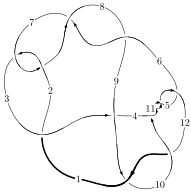
\includegraphics[width=112pt]{../../../GIT/diagram.site/Diagrams/png/1401_12a_0600.png}\\
\ \ \ A knot diagram\footnotemark}&
\allowdisplaybreaks
\textbf{Linearized knot diagam} \\
\cline{2-2}
 &
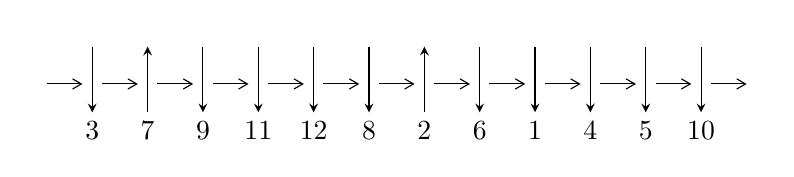
\begin{tikzpicture}[x=20pt, y=17pt]
	% nodes
	\node (C0) at (0, 0) {};
	\node (C1) at (1, 0) {};
	\node (C1U) at (1, +1) {};
	\node (C1D) at (1, -1) {3};

	\node (C2) at (2, 0) {};
	\node (C2U) at (2, +1) {};
	\node (C2D) at (2, -1) {7};

	\node (C3) at (3, 0) {};
	\node (C3U) at (3, +1) {};
	\node (C3D) at (3, -1) {9};

	\node (C4) at (4, 0) {};
	\node (C4U) at (4, +1) {};
	\node (C4D) at (4, -1) {11};

	\node (C5) at (5, 0) {};
	\node (C5U) at (5, +1) {};
	\node (C5D) at (5, -1) {12};

	\node (C6) at (6, 0) {};
	\node (C6U) at (6, +1) {};
	\node (C6D) at (6, -1) {8};

	\node (C7) at (7, 0) {};
	\node (C7U) at (7, +1) {};
	\node (C7D) at (7, -1) {2};

	\node (C8) at (8, 0) {};
	\node (C8U) at (8, +1) {};
	\node (C8D) at (8, -1) {6};

	\node (C9) at (9, 0) {};
	\node (C9U) at (9, +1) {};
	\node (C9D) at (9, -1) {1};

	\node (C10) at (10, 0) {};
	\node (C10U) at (10, +1) {};
	\node (C10D) at (10, -1) {4};

	\node (C11) at (11, 0) {};
	\node (C11U) at (11, +1) {};
	\node (C11D) at (11, -1) {5};

	\node (C12) at (12, 0) {};
	\node (C12U) at (12, +1) {};
	\node (C12D) at (12, -1) {10};
	\node (C13) at (13, 0) {};

	% arrows
	\draw[->,>={angle 60}]
	(C0) edge (C1) (C1) edge (C2) (C2) edge (C3) (C3) edge (C4) (C4) edge (C5) (C5) edge (C6) (C6) edge (C7) (C7) edge (C8) (C8) edge (C9) (C9) edge (C10) (C10) edge (C11) (C11) edge (C12) (C12) edge (C13) ;	\draw[->,>=stealth]
	(C1U) edge (C1D) (C2D) edge (C2U) (C3U) edge (C3D) (C4U) edge (C4D) (C5U) edge (C5D) (C6U) edge (C6D) (C7D) edge (C7U) (C8U) edge (C8D) (C9U) edge (C9D) (C10U) edge (C10D) (C11U) edge (C11D) (C12U) edge (C12D) ;
	\end{tikzpicture} \\
\hhline{~~} \\& 
\textbf{Solving Sequence} \\ \cline{2-2} 
 &
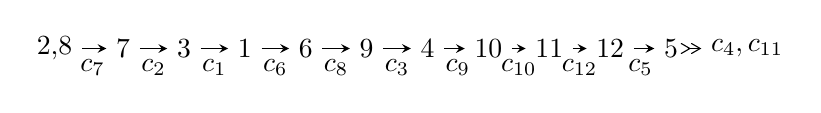
\begin{tikzpicture}[x=22pt, y=7pt]
	% node
	\node (A0) at (-1/8, 0) {2,8};
	\node (A1) at (1, 0) {7};
	\node (A2) at (2, 0) {3};
	\node (A3) at (3, 0) {1};
	\node (A4) at (4, 0) {6};
	\node (A5) at (5, 0) {9};
	\node (A6) at (6, 0) {4};
	\node (A7) at (7, 0) {10};
	\node (A8) at (8, 0) {11};
	\node (A9) at (9, 0) {12};
	\node (A10) at (10, 0) {5};
	\node (C1) at (1/2, -1) {$c_{7}$};
	\node (C2) at (3/2, -1) {$c_{2}$};
	\node (C3) at (5/2, -1) {$c_{1}$};
	\node (C4) at (7/2, -1) {$c_{6}$};
	\node (C5) at (9/2, -1) {$c_{8}$};
	\node (C6) at (11/2, -1) {$c_{3}$};
	\node (C7) at (13/2, -1) {$c_{9}$};
	\node (C8) at (15/2, -1) {$c_{10}$};
	\node (C9) at (17/2, -1) {$c_{12}$};
	\node (C10) at (19/2, -1) {$c_{5}$};
	\node (A11) at (45/4, 0) {$c_{4},c_{11}$};

	% edge
	\draw[->,>=stealth]	
	(A0) edge (A1) (A1) edge (A2) (A2) edge (A3) (A3) edge (A4) (A4) edge (A5) (A5) edge (A6) (A6) edge (A7) (A7) edge (A8) (A8) edge (A9) (A9) edge (A10) ;
	\draw[->>,>={angle 60}]	
	(A10) edge (A11);
\end{tikzpicture} \\ 

\end{tabular} \\

\footnotetext{
The image of knot diagram is generated by the software ``\textbf{Draw programme}" developed by Andrew Bartholomew(\url{http://www.layer8.co.uk/maths/draw/index.htm\#Running-draw}), where we modified some parts for our purpose(\url{https://github.com/CATsTAILs/LinksPainter}).
}\phantom \\ \newline 
\centering \textbf{Ideals for irreducible components\footnotemark of $X_{\text{par}}$} 
 
\begin{align*}
I^u_{1}&=\langle 
u^{54}+u^{53}+\cdots- u-1\rangle \\
\\
\end{align*}
\raggedright * 1 irreducible components of $\dim_{\mathbb{C}}=0$, with total 54 representations.\\
\footnotetext{All coefficients of polynomials are rational numbers. But the coefficients are sometimes approximated in decimal forms when there is not enough margin.}
\newpage
\renewcommand{\arraystretch}{1}
\centering \section*{I. $I^u_{1}= \langle u^{54}+u^{53}+\cdots- u-1 \rangle$}
\flushleft \textbf{(i) Arc colorings}\\
\begin{tabular}{m{7pt} m{180pt} m{7pt} m{180pt} }
\flushright $a_{2}=$&$\begin{pmatrix}0\\u\end{pmatrix}$ \\
\flushright $a_{8}=$&$\begin{pmatrix}1\\0\end{pmatrix}$ \\
\flushright $a_{7}=$&$\begin{pmatrix}1\\u^2\end{pmatrix}$ \\
\flushright $a_{3}=$&$\begin{pmatrix}u\\u^3+u\end{pmatrix}$ \\
\flushright $a_{1}=$&$\begin{pmatrix}u^3\\u^5+u^3+u\end{pmatrix}$ \\
\flushright $a_{6}=$&$\begin{pmatrix}u^2+1\\u^2\end{pmatrix}$ \\
\flushright $a_{9}=$&$\begin{pmatrix}u^4+u^2+1\\u^4\end{pmatrix}$ \\
\flushright $a_{4}=$&$\begin{pmatrix}- u^{11}-2 u^9-4 u^7-4 u^5-3 u^3\\- u^{11}- u^9-2 u^7- u^5+u^3+u\end{pmatrix}$ \\
\flushright $a_{10}=$&$\begin{pmatrix}u^{12}+u^{10}+3 u^8+2 u^6+2 u^4+u^2+1\\u^{14}+2 u^{12}+5 u^{10}+6 u^8+6 u^6+4 u^4+u^2\end{pmatrix}$ \\
\flushright $a_{11}=$&$\begin{pmatrix}- u^{36}-5 u^{34}+\cdots+u^2+1\\- u^{36}-4 u^{34}+\cdots+7 u^4+2 u^2\end{pmatrix}$ \\
\flushright $a_{12}=$&$\begin{pmatrix}u^{21}+2 u^{19}+\cdots+4 u^3+u\\u^{23}+3 u^{21}+\cdots+2 u^3+u\end{pmatrix}$ \\
\flushright $a_{5}=$&$\begin{pmatrix}- u^{46}-5 u^{44}+\cdots-6 u^4+1\\- u^{48}-6 u^{46}+\cdots-16 u^6-4 u^4\end{pmatrix}$\\&\end{tabular}
\flushleft \textbf{(ii) Obstruction class $= -1$}\\~\\
\flushleft \textbf{(iii) Cusp Shapes $= 4 u^{52}+4 u^{51}+\cdots-4 u-10$}\\~\\
\newpage\renewcommand{\arraystretch}{1}
\flushleft \textbf{(iv) u-Polynomials at the component}\newline \\
\begin{tabular}{m{50pt}|m{274pt}}
Crossings & \hspace{64pt}u-Polynomials at each crossing \\
\hline $$\begin{aligned}c_{1},c_{6},c_{8}\end{aligned}$$&$\begin{aligned}
&u^{54}+13 u^{53}+\cdots- u+1
\end{aligned}$\\
\hline $$\begin{aligned}c_{2},c_{7}\end{aligned}$$&$\begin{aligned}
&u^{54}+u^{53}+\cdots- u-1
\end{aligned}$\\
\hline $$\begin{aligned}c_{3}\end{aligned}$$&$\begin{aligned}
&u^{54}+u^{53}+\cdots-947 u-457
\end{aligned}$\\
\hline $$\begin{aligned}c_{4},c_{5},c_{10}\\c_{11}\end{aligned}$$&$\begin{aligned}
&u^{54}- u^{53}+\cdots-3 u-1
\end{aligned}$\\
\hline $$\begin{aligned}c_{9},c_{12}\end{aligned}$$&$\begin{aligned}
&u^{54}-9 u^{53}+\cdots+607 u-89
\end{aligned}$\\
\hline
\end{tabular}\\~\\
\newpage\renewcommand{\arraystretch}{1}
\flushleft \textbf{(v) Riley Polynomials at the component}\newline \\
\begin{tabular}{m{50pt}|m{274pt}}
Crossings & \hspace{64pt}Riley Polynomials at each crossing \\
\hline $$\begin{aligned}c_{1},c_{6},c_{8}\end{aligned}$$&$\begin{aligned}
&y^{54}+57 y^{53}+\cdots-45 y+1
\end{aligned}$\\
\hline $$\begin{aligned}c_{2},c_{7}\end{aligned}$$&$\begin{aligned}
&y^{54}+13 y^{53}+\cdots- y+1
\end{aligned}$\\
\hline $$\begin{aligned}c_{3}\end{aligned}$$&$\begin{aligned}
&y^{54}+17 y^{53}+\cdots+468707 y+208849
\end{aligned}$\\
\hline $$\begin{aligned}c_{4},c_{5},c_{10}\\c_{11}\end{aligned}$$&$\begin{aligned}
&y^{54}-59 y^{53}+\cdots- y+1
\end{aligned}$\\
\hline $$\begin{aligned}c_{9},c_{12}\end{aligned}$$&$\begin{aligned}
&y^{54}+37 y^{53}+\cdots+87587 y+7921
\end{aligned}$\\
\hline
\end{tabular}\\~\\
\newpage\flushleft \textbf{(vi) Complex Volumes and Cusp Shapes}
$$\begin{array}{c|c|c}  
\text{Solutions to }I^u_{1}& \I (\text{vol} + \sqrt{-1}CS) & \text{Cusp shape}\\
 \hline 
\begin{aligned}
u &= \phantom{-}0.421756 + 0.905386 I\end{aligned}
 & \phantom{-}1.46770 + 2.75588 I & -6.58826 - 3.20175 I \\ \hline\begin{aligned}
u &= \phantom{-}0.421756 - 0.905386 I\end{aligned}
 & \phantom{-}1.46770 - 2.75588 I & -6.58826 + 3.20175 I \\ \hline\begin{aligned}
u &= -0.472307 + 0.861794 I\end{aligned}
 & -4.61385 - 0.50041 I & -9.83076 + 3.29327 I \\ \hline\begin{aligned}
u &= -0.472307 - 0.861794 I\end{aligned}
 & -4.61385 + 0.50041 I & -9.83076 - 3.29327 I \\ \hline\begin{aligned}
u &= \phantom{-}0.266117 + 0.940879 I\end{aligned}
 & -10.82780 + 2.68050 I & -17.4218 - 4.4521 I \\ \hline\begin{aligned}
u &= \phantom{-}0.266117 - 0.940879 I\end{aligned}
 & -10.82780 - 2.68050 I & -17.4218 + 4.4521 I \\ \hline\begin{aligned}
u &= -0.407861 + 0.938268 I\end{aligned}
 & \phantom{-}0.96567 - 6.61313 I & -8.59494 + 9.79780 I \\ \hline\begin{aligned}
u &= -0.407861 - 0.938268 I\end{aligned}
 & \phantom{-}0.96567 + 6.61313 I & -8.59494 - 9.79780 I \\ \hline\begin{aligned}
u &= \phantom{-}0.399116 + 0.961261 I\end{aligned}
 & -6.09084 + 9.22771 I & -12.2957 - 8.4163 I \\ \hline\begin{aligned}
u &= \phantom{-}0.399116 - 0.961261 I\end{aligned}
 & -6.09084 - 9.22771 I & -12.2957 + 8.4163 I \\ \hline\begin{aligned}
u &= \phantom{-}0.090589 + 0.936330 I\end{aligned}
 & -7.81225 - 3.84764 I & -15.8715 + 2.0065 I \\ \hline\begin{aligned}
u &= \phantom{-}0.090589 - 0.936330 I\end{aligned}
 & -7.81225 + 3.84764 I & -15.8715 - 2.0065 I \\ \hline\begin{aligned}
u &= -0.276477 + 0.881238 I\end{aligned}
 & -3.10584 - 2.34442 I & -16.9541 + 6.0409 I \\ \hline\begin{aligned}
u &= -0.276477 - 0.881238 I\end{aligned}
 & -3.10584 + 2.34442 I & -16.9541 - 6.0409 I \\ \hline\begin{aligned}
u &= -0.062430 + 0.882605 I\end{aligned}
 & -0.88339 + 1.63649 I & -12.53411 - 3.84361 I \\ \hline\begin{aligned}
u &= -0.062430 - 0.882605 I\end{aligned}
 & -0.88339 - 1.63649 I & -12.53411 + 3.84361 I \\ \hline\begin{aligned}
u &= -0.802323 + 0.832262 I\end{aligned}
 & -4.20575 + 0.66399 I & -10.65156 + 0. I\phantom{ +0.000000I} \\ \hline\begin{aligned}
u &= -0.802323 - 0.832262 I\end{aligned}
 & -4.20575 - 0.66399 I & -10.65156 + 0. I\phantom{ +0.000000I} \\ \hline\begin{aligned}
u &= \phantom{-}0.818373 + 0.865309 I\end{aligned}
 & \phantom{-}3.46423 + 0.45809 I & -8.00000 + 0. I\phantom{ +0.000000I} \\ \hline\begin{aligned}
u &= \phantom{-}0.818373 - 0.865309 I\end{aligned}
 & \phantom{-}3.46423 - 0.45809 I & -8.00000 + 0. I\phantom{ +0.000000I} \\ \hline\begin{aligned}
u &= -0.823200 + 0.900365 I\end{aligned}
 & \phantom{-}5.63050 - 3.07356 I & \phantom{-0.000000 } 0 \\ \hline\begin{aligned}
u &= -0.823200 - 0.900365 I\end{aligned}
 & \phantom{-}5.63050 + 3.07356 I & \phantom{-0.000000 } 0 \\ \hline\begin{aligned}
u &= -0.886232 + 0.838665 I\end{aligned}
 & \phantom{-}2.20397 + 6.81927 I & \phantom{-0.000000 } 0 \\ \hline\begin{aligned}
u &= -0.886232 - 0.838665 I\end{aligned}
 & \phantom{-}2.20397 - 6.81927 I & \phantom{-0.000000 } 0 \\ \hline\begin{aligned}
u &= -0.782939 + 0.941062 I\end{aligned}
 & -4.53436 - 6.62284 I & \phantom{-0.000000 } 0 \\ \hline\begin{aligned}
u &= -0.782939 - 0.941062 I\end{aligned}
 & -4.53436 + 6.62284 I & \phantom{-0.000000 } 0 \\ \hline\begin{aligned}
u &= \phantom{-}0.883660 + 0.847398 I\end{aligned}
 & \phantom{-}9.22964 - 3.95082 I & \phantom{-0.000000 } 0 \\ \hline\begin{aligned}
u &= \phantom{-}0.883660 - 0.847398 I\end{aligned}
 & \phantom{-}9.22964 + 3.95082 I & \phantom{-0.000000 } 0 \\ \hline\begin{aligned}
u &= \phantom{-}0.803804 + 0.926221 I\end{aligned}
 & \phantom{-}3.27760 + 5.61427 I & \phantom{-0.000000 } 0 \\ \hline\begin{aligned}
u &= \phantom{-}0.803804 - 0.926221 I\end{aligned}
 & \phantom{-}3.27760 - 5.61427 I & \phantom{-0.000000 } 0\\
 \hline 
 \end{array}$$\newpage$$\begin{array}{c|c|c}  
\text{Solutions to }I^u_{1}& \I (\text{vol} + \sqrt{-1}CS) & \text{Cusp shape}\\
 \hline 
\begin{aligned}
u &= -0.880738 + 0.857162 I\end{aligned}
 & \phantom{-}9.69162 - 0.23278 I & \phantom{-0.000000 } 0 \\ \hline\begin{aligned}
u &= -0.880738 - 0.857162 I\end{aligned}
 & \phantom{-}9.69162 + 0.23278 I & \phantom{-0.000000 } 0 \\ \hline\begin{aligned}
u &= \phantom{-}0.878437 + 0.871151 I\end{aligned}
 & \phantom{-}3.67628 + 3.01982 I & \phantom{-0.000000 } 0 \\ \hline\begin{aligned}
u &= \phantom{-}0.878437 - 0.871151 I\end{aligned}
 & \phantom{-}3.67628 - 3.01982 I & \phantom{-0.000000 } 0 \\ \hline\begin{aligned}
u &= -0.610477 + 0.439255 I\end{aligned}
 & -3.29528 - 3.49644 I & -6.18778 + 3.39542 I \\ \hline\begin{aligned}
u &= -0.610477 - 0.439255 I\end{aligned}
 & -3.29528 + 3.49644 I & -6.18778 - 3.39542 I \\ \hline\begin{aligned}
u &= \phantom{-}0.229939 + 0.699250 I\end{aligned}
 & -0.424354 + 1.032670 I & -6.76973 - 6.18966 I \\ \hline\begin{aligned}
u &= \phantom{-}0.229939 - 0.699250 I\end{aligned}
 & -0.424354 - 1.032670 I & -6.76973 + 6.18966 I \\ \hline\begin{aligned}
u &= \phantom{-}0.844032 + 0.951939 I\end{aligned}
 & \phantom{-}3.41989 + 3.36125 I & \phantom{-0.000000 } 0 \\ \hline\begin{aligned}
u &= \phantom{-}0.844032 - 0.951939 I\end{aligned}
 & \phantom{-}3.41989 - 3.36125 I & \phantom{-0.000000 } 0 \\ \hline\begin{aligned}
u &= -0.836819 + 0.962125 I\end{aligned}
 & \phantom{-}9.35926 - 6.13178 I & \phantom{-0.000000 } 0 \\ \hline\begin{aligned}
u &= -0.836819 - 0.962125 I\end{aligned}
 & \phantom{-}9.35926 + 6.13178 I & \phantom{-0.000000 } 0 \\ \hline\begin{aligned}
u &= \phantom{-}0.832840 + 0.969452 I\end{aligned}
 & \phantom{-}8.84361 + 10.31070 I & \phantom{-0.000000 } 0 \\ \hline\begin{aligned}
u &= \phantom{-}0.832840 - 0.969452 I\end{aligned}
 & \phantom{-}8.84361 - 10.31070 I & \phantom{-0.000000 } 0 \\ \hline\begin{aligned}
u &= -0.829260 + 0.975631 I\end{aligned}
 & \phantom{-}1.77109 - 13.17440 I & \phantom{-0.000000 } 0 \\ \hline\begin{aligned}
u &= -0.829260 - 0.975631 I\end{aligned}
 & \phantom{-}1.77109 + 13.17440 I & \phantom{-0.000000 } 0 \\ \hline\begin{aligned}
u &= \phantom{-}0.596016 + 0.373336 I\end{aligned}
 & \phantom{-}3.12910 + 1.02645 I & -2.02831 - 3.48790 I \\ \hline\begin{aligned}
u &= \phantom{-}0.596016 - 0.373336 I\end{aligned}
 & \phantom{-}3.12910 - 1.02645 I & -2.02831 + 3.48790 I \\ \hline\begin{aligned}
u &= \phantom{-}0.635066 + 0.277401 I\end{aligned}
 & -3.94406 - 5.44870 I & -6.82965 + 3.24384 I \\ \hline\begin{aligned}
u &= \phantom{-}0.635066 - 0.277401 I\end{aligned}
 & -3.94406 + 5.44870 I & -6.82965 - 3.24384 I \\ \hline\begin{aligned}
u &= -0.610761 + 0.317401 I\end{aligned}
 & \phantom{-}2.90528 + 2.85235 I & -2.90911 - 4.01001 I \\ \hline\begin{aligned}
u &= -0.610761 - 0.317401 I\end{aligned}
 & \phantom{-}2.90528 - 2.85235 I & -2.90911 + 4.01001 I \\ \hline\begin{aligned}
u &= \phantom{-}0.540222\phantom{ +0.000000I}\end{aligned}
 & -8.09120\phantom{ +0.000000I} & -10.3100\phantom{ +0.000000I} \\ \hline\begin{aligned}
u &= -0.376064\phantom{ +0.000000I}\end{aligned}
 & -0.895266\phantom{ +0.000000I} & -10.7040\phantom{ +0.000000I}\\
 \hline 
 \end{array}$$\newpage
\newpage\renewcommand{\arraystretch}{1}
\centering \section*{ II. u-Polynomials}
\begin{tabular}{m{50pt}|m{274pt}}
Crossings & \hspace{64pt}u-Polynomials at each crossing \\
\hline $$\begin{aligned}c_{1},c_{6},c_{8}\end{aligned}$$&$\begin{aligned}
&u^{54}+13 u^{53}+\cdots- u+1
\end{aligned}$\\
\hline $$\begin{aligned}c_{2},c_{7}\end{aligned}$$&$\begin{aligned}
&u^{54}+u^{53}+\cdots- u-1
\end{aligned}$\\
\hline $$\begin{aligned}c_{3}\end{aligned}$$&$\begin{aligned}
&u^{54}+u^{53}+\cdots-947 u-457
\end{aligned}$\\
\hline $$\begin{aligned}c_{4},c_{5},c_{10}\\c_{11}\end{aligned}$$&$\begin{aligned}
&u^{54}- u^{53}+\cdots-3 u-1
\end{aligned}$\\
\hline $$\begin{aligned}c_{9},c_{12}\end{aligned}$$&$\begin{aligned}
&u^{54}-9 u^{53}+\cdots+607 u-89
\end{aligned}$\\
\hline
\end{tabular}\newpage\renewcommand{\arraystretch}{1}
\centering \section*{ III. Riley Polynomials}
\begin{tabular}{m{50pt}|m{274pt}}
Crossings & \hspace{64pt}Riley Polynomials at each crossing \\
\hline $$\begin{aligned}c_{1},c_{6},c_{8}\end{aligned}$$&$\begin{aligned}
&y^{54}+57 y^{53}+\cdots-45 y+1
\end{aligned}$\\
\hline $$\begin{aligned}c_{2},c_{7}\end{aligned}$$&$\begin{aligned}
&y^{54}+13 y^{53}+\cdots- y+1
\end{aligned}$\\
\hline $$\begin{aligned}c_{3}\end{aligned}$$&$\begin{aligned}
&y^{54}+17 y^{53}+\cdots+468707 y+208849
\end{aligned}$\\
\hline $$\begin{aligned}c_{4},c_{5},c_{10}\\c_{11}\end{aligned}$$&$\begin{aligned}
&y^{54}-59 y^{53}+\cdots- y+1
\end{aligned}$\\
\hline $$\begin{aligned}c_{9},c_{12}\end{aligned}$$&$\begin{aligned}
&y^{54}+37 y^{53}+\cdots+87587 y+7921
\end{aligned}$\\
\hline
\end{tabular}
\vskip 2pc
\end{document}